% TeX encoding = utf8
% TeX spellcheck = pl_PL 
\documentclass[a4paper,titlepage,11pt,twosides,floatssmall]{mwrep}
\usepackage[left=2.5cm,right=2.5cm,top=2.5cm,bottom=2.5cm]{geometry}
\usepackage[OT1]{fontenc}
\usepackage{polski}
\usepackage{amsmath}
\usepackage{amsfonts}
\usepackage{amssymb}
\usepackage{graphicx}
\usepackage{url}
\usepackage{tikz}
\usetikzlibrary{arrows,calc,decorations.markings,math,arrows.meta}
\usepackage{rotating}
\usepackage[percent]{overpic}
\usepackage[utf8]{inputenc}
\usepackage{xcolor}
\usepackage{pgfplots}
\usetikzlibrary{pgfplots.groupplots}
\usepackage{listings}
\usepackage{matlab-prettifier}
\usepackage{siunitx}
\usepackage[section]{placeins}
\definecolor{szary}{rgb}{0.95,0.95,0.95}
\SendSettingsToPgf
\sisetup{detect-weight,exponent-product=\cdot,output-decimal-marker={,},per-mode=symbol,binary-units=true,range-phrase={-},range-units=single}

%konfiguracje pakietu listings
\lstset{
	backgroundcolor=\color{szary},
	frame=single,
	breaklines=true,
}
\lstdefinestyle{customlatex}{
	basicstyle=\footnotesize\ttfamily,
	%basicstyle=\small\ttfamily,
}
\lstdefinestyle{customc}{
	breaklines=true,
	frame=tb,
	language=C,
	xleftmargin=0pt,
	showstringspaces=false,
	basicstyle=\small\ttfamily,
	keywordstyle=\bfseries\color{green!40!black},
	commentstyle=\itshape\color{purple!40!black},
	identifierstyle=\color{blue},
	stringstyle=\color{orange},
}
\lstdefinestyle{custommatlab}{
	captionpos=t,
	breaklines=true,
	frame=tb,
	xleftmargin=0pt,
	language=matlab,
	showstringspaces=false,
	%basicstyle=\footnotesize\ttfamily,
	basicstyle=\scriptsize\ttfamily,
	keywordstyle=\bfseries\color{green!40!black},
	commentstyle=\itshape\color{purple!40!black},
	identifierstyle=\color{blue},
	stringstyle=\color{orange},
}

%wymiar tekstu (bez żywej paginy)
\textwidth 160mm \textheight 247mm

%ustawienia pakietu pgfplots
\pgfplotsset{
	tick label style={font=\scriptsize},
	label style={font=\small},
	legend style={font=\small},
	title style={font=\small}
}

\def\figurename{Rys.}
\def\tablename{Tab.}

%konfiguracja liczby pływających elementów
\setcounter{topnumber}{0}%2
\setcounter{bottomnumber}{3}%1
\setcounter{totalnumber}{5}%3
\renewcommand{\textfraction}{0.01}%0.2
\renewcommand{\topfraction}{0.95}%0.7
\renewcommand{\bottomfraction}{0.95}%0.3
\renewcommand{\floatpagefraction}{0.35}%0.5

\begin{document}
	
	\begin{titlepage}
		\begin{center}
			\Huge{\textsc{Sprawozdanie z pierwszego projektu z przedmiotu \\,,Sztuczna Inteligencja w Automatyce''}} \\
			[15cm]
			\Large{Numer zadania: 10 \\Wykonawcy:}\\
			\Large{Daniel Giełdowski \\ Piort Chachuła}
		\end{center}
	\end{titlepage}
	
	\tableofcontents
	\newpage
	\input{opis.tex}
	\chapter{Zadanie 1}
	\label{ch:z1}
	\begin{equation}
	\left\{
	\begin{tabular}{l}
		$x_1(k)= - \alpha_1 x_1(k-1) + x_2(k-1) + \beta_1 g_1(u(k-3))$ \\\\
		$x_2(k)= - \alpha_2 x_1(k-1) + \beta_2 g_1(u(k-3))$\\\\
		$y(k)=g_2(x_1(k))$\\\\
	\end{tabular}
	\right.
	\label{eq:dyskretne}
	\end{equation}
	gdzie $u$-sygnał wejściowy, $y$-sygnał wyjściowy, $x_1$, $x_2$ - zmienne stanu, $\alpha_1 = -1,422574$, $\alpha_2 = 0,466776$, $\beta_1 = 0,017421$, $\beta_2 = 0,013521$ oraz
	\begin{equation}
		g_1(u(k-3))=\frac{exp(5u(k-3))-1}{exp(5u(k-3))+1}, g_2(x_1(k))=1-exp(-1.5x_1(k))
	\end{equation}
	Punkt pracy $u=y=x_1=x_2=0$, $u^min=-1 : u^max = 1$.
	W wersji statycznej:
	\begin{equation}
		\left\{
		\begin{tabular}{l}
		$x_1= - \alpha_1 x_1+x_2+ \beta_1 g_1(u)$ \\\\
		$x_2= - \alpha_2 x_1+ \beta_2 g_1(u)$\\\\
		$y=g_2(x_1)$\\\\
		\end{tabular}
		\right.
		\label{eq:statyczne}
	\end{equation}
	Po przekształceniach:
	\begin{equation}
		x_1 = \frac{(\beta_1 + \beta_2)g_1(u)}{1+\alpha_1+\alpha_2}
		\label{eq:x1_static}
	\end{equation}
	Podstawieniu równania (\ref{eq:x1_static}) do $y$ otrzymujemy
	\begin{equation}
		y(u) = g_2(\frac{(\beta_1 + \beta_2)g_1(u)}{1+\alpha_1+\alpha_2}
		\label{eq:x1_static})
	\end{equation}
	\chapter{Modelowanie procesu}
	\label{ch:mod}
	
	\section{Opóźnienie}
		\label{sec:tau}
	
	\section{Dobór liczby neuronów}
		\label{sec:neurony}
		
	\section{Model z algorytmu BFGS}
		\label{sec:bfgs}
		
	\section{Symulacja modelu z algorytmu BFGS}
		\label{sec:bfgs_sym}
		
	\section{Model z algorytmu najszybszego spadku}
		\label{sec:naj_sp}
		
	\section{Model z algorytmu BFGS z uczeniem bez rekurencji}
		\label{sec:bfgs_arx}
		
	\section{Symulacja modelu z algorytmu BFGS z uczeniem bez rekurencji}
		\label{sec:bfgs_arx_sym}
		
	\section{Model metodą najmniejszych kwadratów}
		\label{sec:mnk}
	\chapter{Regulacja procesu}
	\label{ch:reg}
	
	\section{Implementacja NPL}
		\label{sec:NPL}
		NPL jest algorytmem regulacji predykcyjnym z nieliniową predykcją i z linearyzacją oznacza to że do wyznaczania trajektori swobodnej (która zależy tylko od przeszłych sterowań) używamy nieliniowego modelu neuronowego:
		\begin{equation}
		\begin{tabular}{l}
		$y^0(k+p|k)=w20+w2*tanh(w10+w1*x(k+p))+dk$
		\end{tabular}
		\label{eq:NPL_y0}
		\end{equation}
		gdzie
		\begin{equation}
		\begin{tabular}{l}
		$dk = y(k)-y^M(k)$
		\end{tabular}
		\label{eq:dk}
		\end{equation}
		\begin{equation}
		\begin{tabular}{l}
		$x(k)=$ $\begin{bmatrix}u(min(k-\tau+p,k-1))\\u(min(k-\tau-1+p,k-1))\\y(k-1+p)\\y(k-2+p)\end{bmatrix}$
		\end{tabular}
		\label{eq:wesn}
		\end{equation}
		$p=$ ilość chwil w przyszłóść.
		Warto dodać, że we wzore \ref{eq:wesn} dla chwil czasu dalszych od $k$ zakłada się że $y(k+p)=y^0(k+p|k)$.\\
		Aby móc rozwiązać algorytm analitycznie dokonuje się linearyzacji wyjścia modelu. Współczynniki $b_3$,$b_4$,$a_1$,$a_2$ we wzorze
		\begin{equation}
		\begin{tabular}{l}
		$y(k)=b_3u(k-\tau)+b_4(k-\tau-1)-a_1y(k-1)-a_2y(k-2)$
		\end{tabular}
		\label{eq:NPL_wyjscielinear}
		\end{equation}
		otrzymuje się poprzez obliczenie pochodnej cząstkowej po odpowiednim wejściu modelu neuronowego. Mając obliczone współczynniki można użyć ich do wyznaczenia odpowiedzi skokowej ze wzoru
		\begin{equation}
		\begin{tabular}{l}
		$s_j(k)=\sum\limits_{i=1}^{min(j,n_B)}b_i(k)-\sum\limits_{i=1}^{min(j-1,n_A)}s_{j-i}(k)$
		\end{tabular}
		\label{eq:NPL_odpowiedzskok}
		\end{equation}
		których można użyć do wypełnienia macierzy dynamicznej M.
		
		\begin{equation}
		\boldsymbol{M}=\left[
		\begin{array}
		{cccc}
		s_{1} & 0 & \ldots & 0\\
		s_{2} & s_{1} & \ldots & 0\\
		\vdots & \vdots & \ddots & \vdots\\
		s_{N} & s_{N-1} & \ldots &  s_{N-N_{\mathrm{u}}+1}
		\end{array}
		\right]_{\mathrm{NxN_u}}
		\label{Mm}
		\end{equation}
		
		Na koniec można obliczyć optymalne przyszłe sterowania(przy zadanych horyzontach predykcji N i sterowania Nu oraz współczynniku kary $\lambda$). 
		\begin{equation}
		\begin{tabular}{l}
		$dU=K*(Y_{zad}(k)-Y^0)$
		\end{tabular}
		\label{eq:NPL_du}
		\end{equation}
		gdzie $Y_{zad}(k)$ to wektor długości N zawierający aktualną wartość zadaną, $Y^0$ to wektor N przyszłych, predykowanych wartości wyjścia oraz
		\begin{equation}
		\begin{tabular}{l}
		$K=(M'*M+\lambda I)^{-1}*M'$
		\end{tabular}
		\label{eq:NPL_K}
		\end{equation}
	
		
		
	\section{Strojenie NPL}
		\label{sec:stroj_NPL}
		Regulator NPL został nastrojony z użyciem sieci neuronowej wytrenowanej algorytmem BFGS z użyciem rekurencji opisanej w sekcji \ref{sec:bfgs}. Strojenie regulatora NPL rozpoczęliśmy od parametrów $N=10$, $N_u=2$ oraz $\lambda=1$. Przebieg dla tych wartości zaprezentowany jest poniżej (rys. \ref{fig:NPL0}). Jak widać już od samego początku przebieg regulacji nie jest zły. Błąd o wartości 75.2963 na 600 próbkach nie jest idealny, ale akceptowalny. Mimo tego działanie regulatora na pewno można poprawić. Wyjście ulega nieznacznym oscylacjom, a sterowanie jest dosyć gwałtowne.
		
		\begin{figure}[h!]
			\centering
			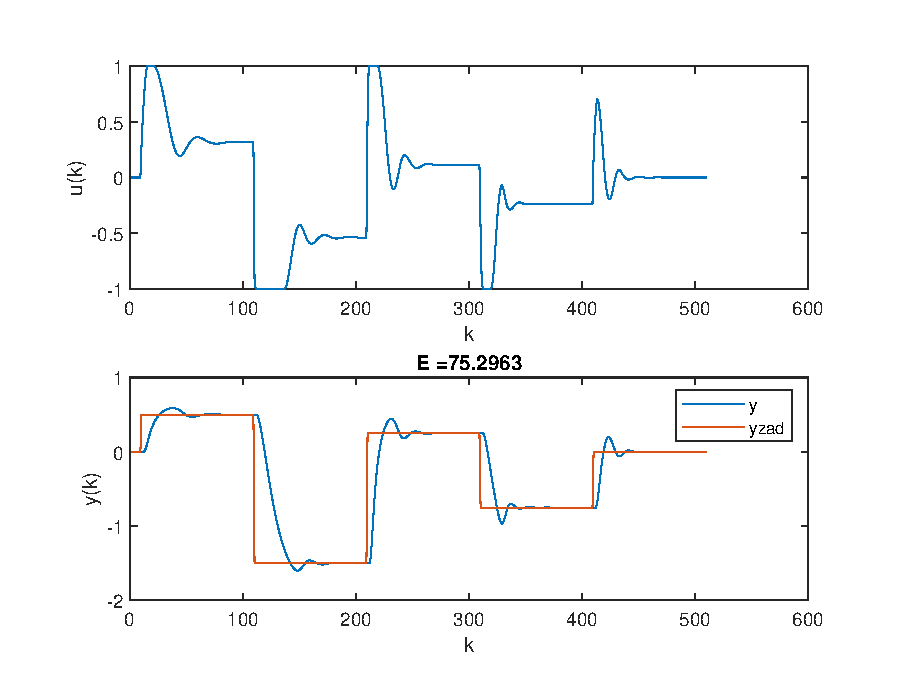
\includegraphics[width=0.7\linewidth]{img/strojenieNPL_N_10_Nu_2_lam_1.eps}
			\caption{Działanie regulatora NPL z nastawami N=10, Nu=2, $\lambda$=1}
			\label{fig:NPL0}
		\end{figure}
		
		Postanowiliśmy zwiększać horyzont predykcji i udało nam się uzyskać lepsze wyniki dla $N=20$ (rys. \ref{fig:NPL1}). Jak widać oscylacje na wyjściu zniknęły, a sterowanie stało się mniej gwałtowne. Spadł też błąd regulacji, do wartości E = 74.8182.
		\begin{figure}[h!]
			\centering
			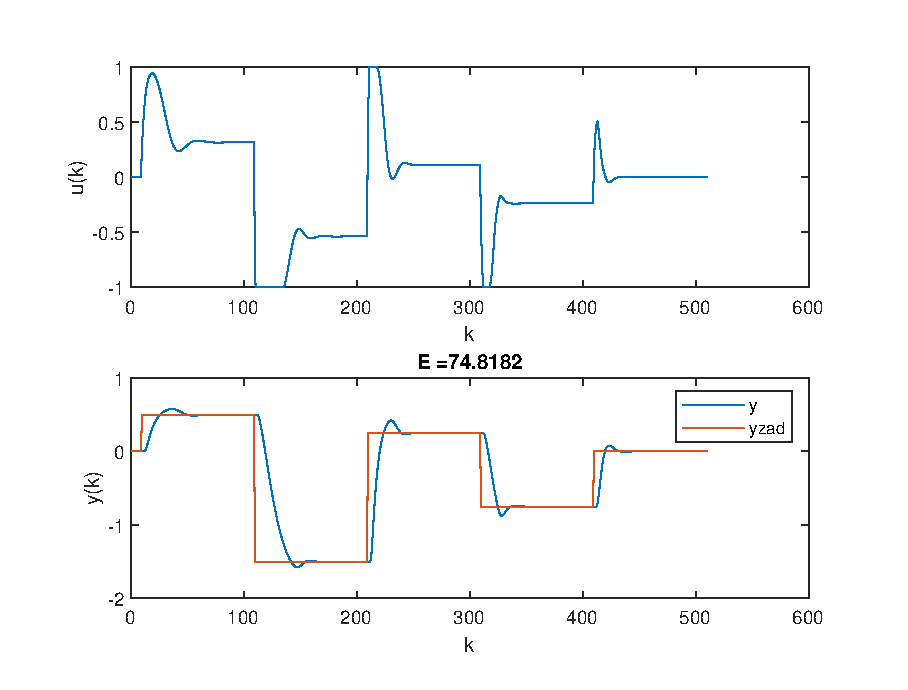
\includegraphics[width=0.7\linewidth]{img/NPLN20.eps}
			\caption{Działanie regulatora NPL z nastawami N=20, Nu=2, $\lambda$=1}
			\label{fig:NPL1}
		\end{figure}
		
		\newpage
		Następnie postanowiliśmy dobrać horyzont sterowania. Niestety zarówno przy zwiększaniu jak i zmniejszaniu horyzunto jakość regulacji pogarszała się, co można zaobserwować na wykresach \ref{fig:NPL2} i \ref{fig:NPL3}. Dla Nu równego 1 błąd regulacji co prawda spadł, a wykres wyjścia wygląda lepiej, ale następują niekontrolowane, ostre skoki sterowania. Dla Nu równego 3 zarówno przebiegi wyjścia jak i wejścia pogarszają się.
		\begin{figure}[h!]
			\centering
			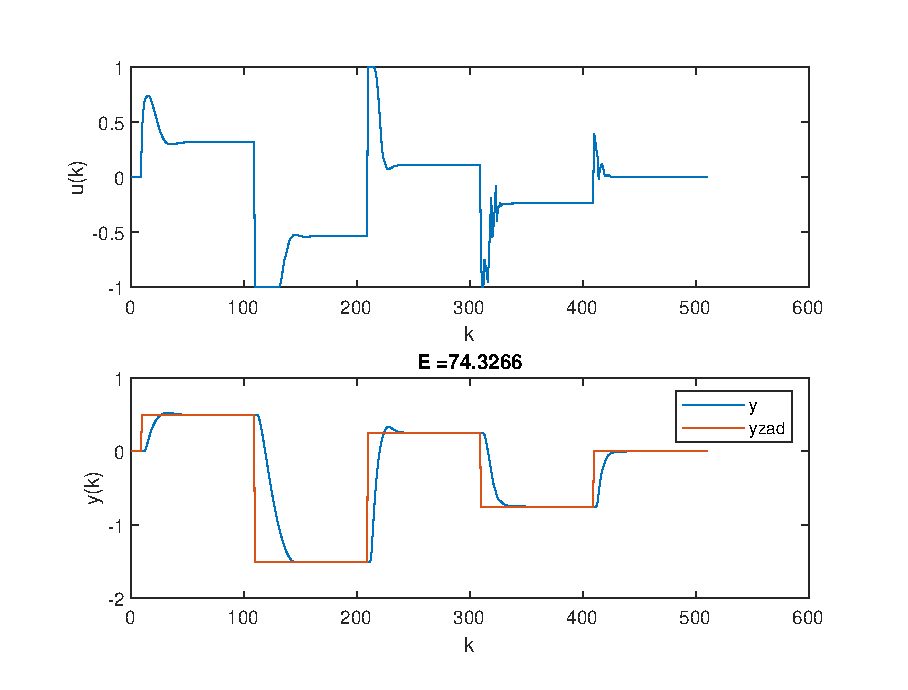
\includegraphics[width=0.7\linewidth]{img/NPLNu1.eps}
			\caption{Działanie regulatora NPL z nastawami N=20, Nu=1, $\lambda$=1}
			\label{fig:NPL2}
		\end{figure}
		
		\begin{figure}[h!]
			\centering
			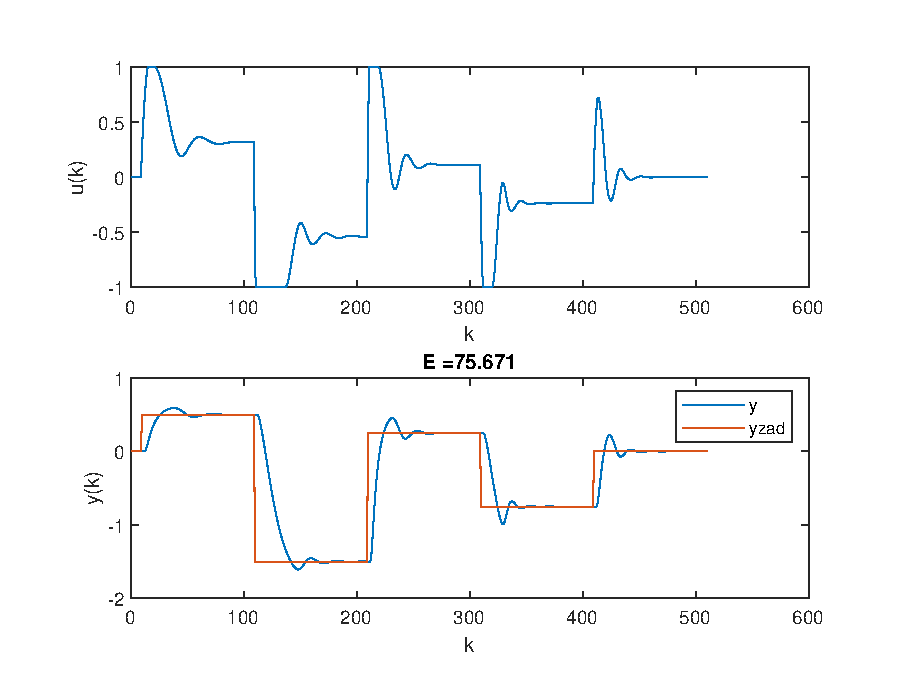
\includegraphics[width=0.7\linewidth]{img/NPLNu3.eps}
			\caption{Działanie regulatora NPL z nastawami N=20, Nu=3, $\lambda$=1}
			\label{fig:NPL3}
		\end{figure}
		
		\newpage
		Mając dobrane $N$ oraz $N_u$ pozostało zbadać wpływ współczynnika $\lambda$. Po zwiększeniu o jeden dało się zaobserwować spadek oscylacji, wygładzenie sterowania i spadek przeregulowania. Z drugiej strony wartość błędu wzrosła, ponieważ złagodzenie sterowania spowodowało nieznaczne spowolnienie regulacji. Postanowiliśmy zostawić $\lambda$ przy obecnej wartości 2, dla której przebieg przedstawiliśmy an wykresie \ref{fig:NPL4}. Dalsze zwiększanie tego parametru, choć zmniejszałoby skoki sterowania mogłoby końcowo doprowadzić do pogorszenia regulacji, ze względu na jej spowolnienie.
		\begin{figure}[h!]
			\centering
			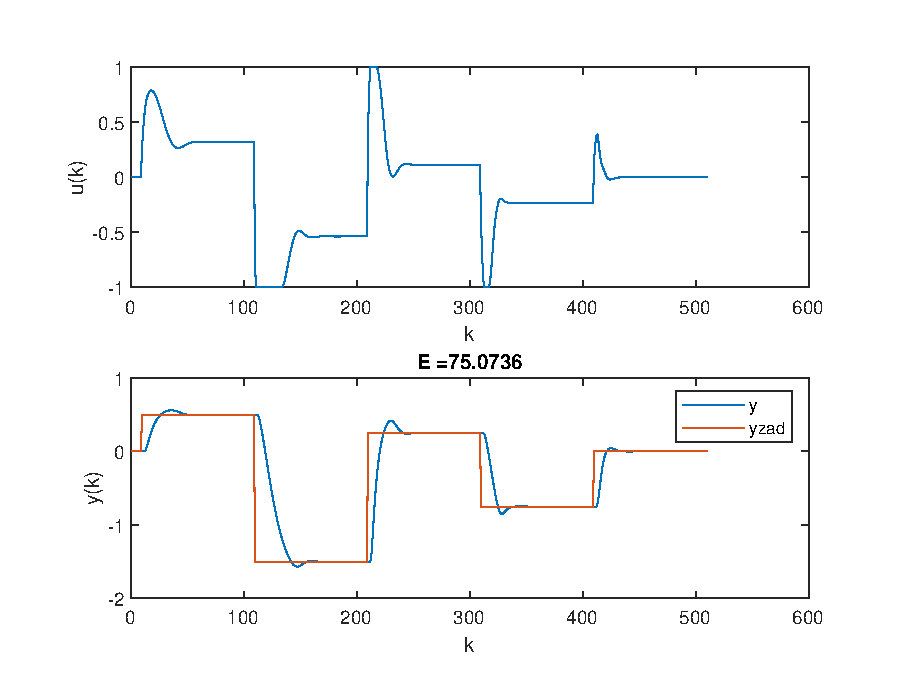
\includegraphics[width=\linewidth]{img/NPLlam2.eps}
			\caption{Działanie regulatora NPL z nastawami N=20, Nu=2, $\lambda$=2}
			\label{fig:NPL4}
		\end{figure}
		
	\newpage	
	\section{GPC}
		\label{sec:GPC}
		Algorytm regulacji GPC, różni się tym od NPL, że na całym horyzocnie predykcji korzysta się z liniowego modelu wyznaczonego metodą najmniejszych kwadratów. Jak można było zauważyć z rys. \ref{fig:mnk} taki model nie gwarantuje najlepszego odwzorowania obiektu, przez co jak można się domyślać jakość regulacji również może być gorsza.
		Do wyznaczania sterowania w wersji analitycznej wyznacza predykcje wyjscia modelu $N$ chwil do przodu ze wzoru
		\begin{equation}
		\begin{tabular}{l}
		$y^0(k+p|k)=b_3u(min(k-3+p,k-1))+b_4u(min(k-4+p),k-1)-a_1y(k-1+p)-a_2y(k-2+p)$
		\end{tabular}
		\label{eq:GPC_y0}
		\end{equation}
		oraz analogicznie do wzoru \ref{eq:NPL_y0} $y(k+p)=y^0(k+p|k)$. Parametry $a_i$ oraz $b_i$ otrzymywane są z metody najmniejszych kwadratów. Macierz dynamiczna jest stała i wyznaczana przy użyciu odpowiedzi skokowej ze wzoru \ref{eq:NPL_odpowiedzskok}. Na wykresie poniżej można zauważyć, że jakość regulacji w istocie pozostawia wiele do życzenia (rys \ref{fig:GPC}).
		
		\begin{figure}[h!]
			\centering
			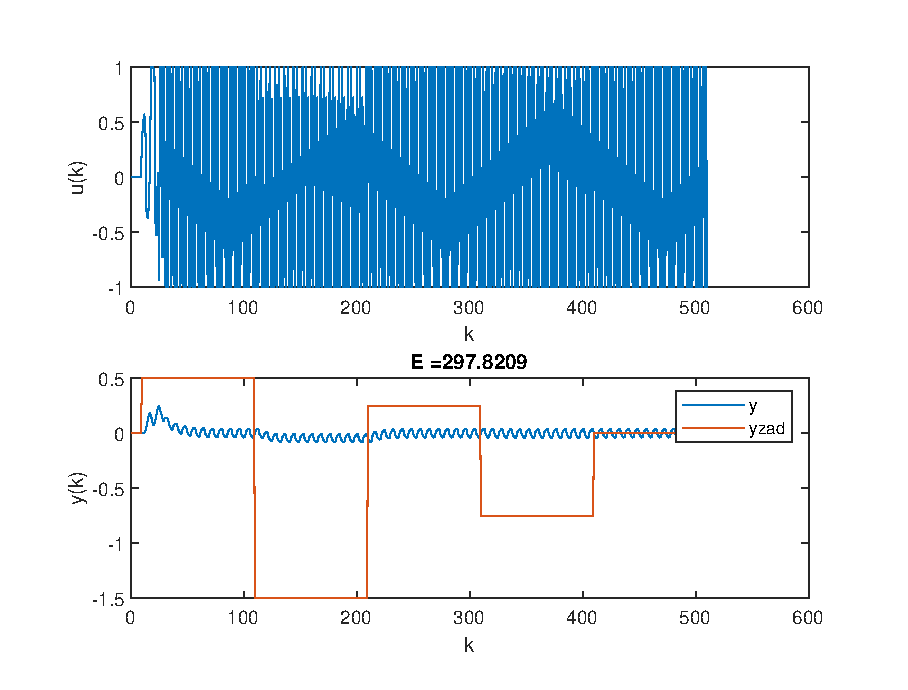
\includegraphics[width=\linewidth]{img/GPC.eps}
			\caption{Działanie regulatora GPC z nastawami N=20, Nu=2, $\lambda$=2}
			\label{fig:GPC}
		\end{figure}
	
		\newpage
		Należy wziąć pod uwagę, że przez silną nieliniowość obiektu, liniowy algorytm GPC może generować duże sterowania, które po nałożeniu ograniczeń wprowadzą obiekt w stałe oscylacje. Można temu zapobiec poprzez zwiększenie współczynnika $\lambda$ o parę rzędów wielkości. Na rys. \ref{fig:GPC100} można zobaczyć, że jakość regulacji polepszyła się, lecz mimo to sterowanie wciąż jest zbyt ostre, a czas regulacji wolniejszy niż w przypadku NPL. W dodatku zarówno dla sterowania jak i wyjścia występują widoczne oscylacje.
		\begin{figure}[h!]
			\centering
			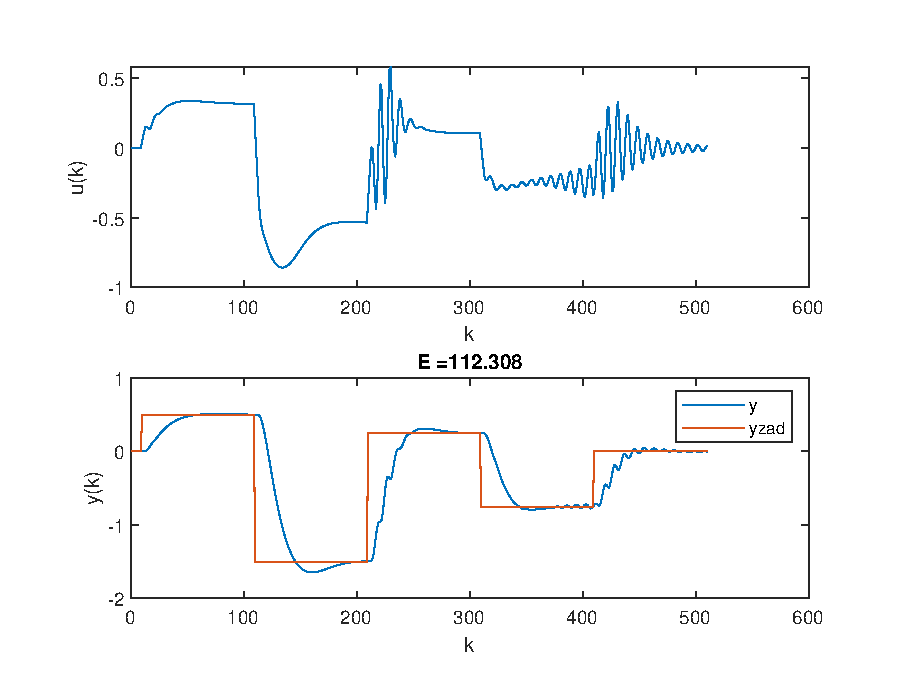
\includegraphics[width=\linewidth]{img/GPC100.eps}
			\caption{Działanie regulatora GPC z nastawami N=20, Nu=2, $\lambda$=100}
			\label{fig:GPC100}
		\end{figure}
	\chapter{Zadania dodatkowe}
	\label{ch:dod}
	\section{PID}
		\label{sec:PID}
		Algorytm PID oblicze przyszłe sterowanie na podstawie wartości, pochodnej i całki uchybu w odpowiednich proporcjach. Popularną sposobem strojenia tego regulatora jest metoda Zieglera-Nicholsa, która polega na doprowadzenie obiektu na granice stabilności przy wyłączonych członach I oraz D, zmierzenia okresu drgań a następnie podstawieniu odpowiednich wartości do wzoru. W przypadku obiektu z zadania obiekt był na granicy stabilności (w we wszystkich zadanych przez nas punktach pracy) przy $K_p=4$, co można zaobserwować na rys. \ref{fig:PID0}.
		
		\begin{figure}[h!]
			\centering
			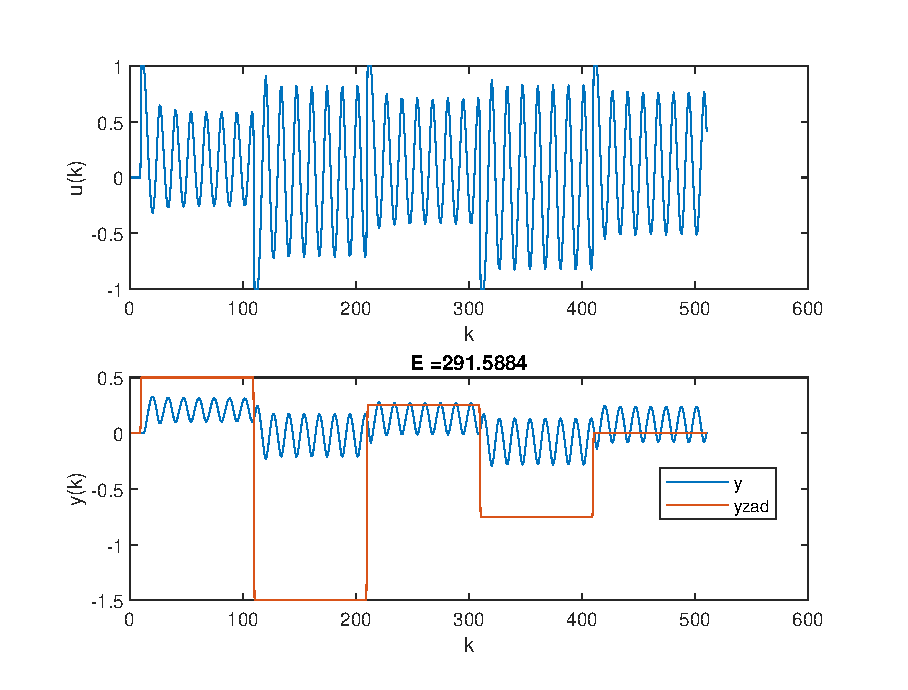
\includegraphics[width=\linewidth]{img/strojeniePID_Kp_4_Ti_duzo_Td_0.eps}
			\caption{Działanie regulatora PID z nastawami Kp = 4, Ti = Inf, Td = 0}
			\label{fig:PID0}
		\end{figure}
		
		\newpage
		Następnie, po podstawieniu zmierzonych wartości (okres drgań $T_u=13$) otrzymaliśmy przebieg przedstawiony na rys. \ref{fig:PID1}.
		Widać, że regulator próbuje naśladować przebieg wartości zadanej, i robi to nie najgorzej (mimo bardzo ostrego sterowania), lecz dla niektórych punktów pracy pojawiają się niegasnące oscylacje. Nastrojony w ten sposób regulator wydaje się dobrze radzić sobie w bliskości granicy przedziału sterowania, a gorzej będąc w jego centrum.
		
		\begin{figure}[h!]
			\centering
			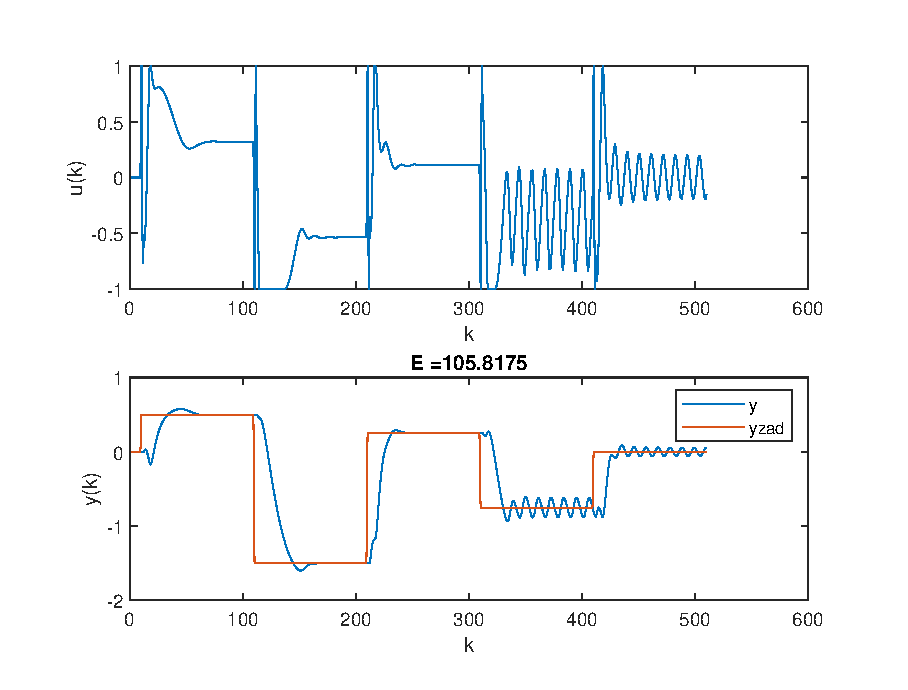
\includegraphics[width=\linewidth]{img/strojeniePID_Ziegler_Nichols.eps}
			\caption{Działanie regulatora PID z nastawami Kp = 2.4, Ti = 6.5, Td = 1.625}
			\label{fig:PID1}
		\end{figure}
		
		\newpage
	\section{NO}
		\label{sec:NO}
		Algorytm NO, tym różni się od algorytmu NPL, że do wyznaczania predykcji wyjścia stosuje się model nieliniowy. Oznacza to, że nie można wyznaczyć przyszłych sterowań analitycznie. Posługując się wskaznikiem jakości
		\begin{equation}
		\begin{tabular}{l}
		$J(k) = \sum\limits_{p=1}^{N}(y^{zad}(k)-\hat{y}(k+p|k))^2+\lambda\sum\limits_{p=0}^{N_u}(\Delta u(k+p|k))^2$
		\end{tabular}
		\label{eq:wsk_jakosc}
		\end{equation}
		wyznacza się takie sterowania dla których jest on najmniejszy.
		Wyliczyjąć predykcje wyjścia jako
		\begin{equation}
		\begin{tabular}{l}
		$\hat{y}(k+p|k)=w20 + w2*tanh(w10+w1*x(k+p|k))+dk$
		\end{tabular}
		\label{eq:NO_wyjscie}
		\end{equation}
		gdzie
		\begin{equation}
		\begin{tabular}{l}
		$x(k+p|k)=\begin{bmatrix}u(k-3+p)\\u(k-4+p)\\y(k-1+p)\\y(k-2+p)\end{bmatrix}$
		\end{tabular}
		\label{eq:NO_wesn}
		\end{equation}
		We wzorze tym, podobnie jak w równaniu \ref{eq:NPL_y0} i \ref{eq:GPC_y0} dla $y(k+p|k)=\hat{y}(k+p|k)$. Dodatkowo, ponieważ przewidujemy jedynie przez cały horyzont sterowania, zakłada się, że sterowanie dla $p>Nu-1$ przyjmuje wartość $u(k+p)=u(k+N_u-1)$. Mając wyznaczone wszystkie wartości można obliczyć zadanie optymalizacji. W tym celu wykorzystaliśmy obecny w Matlabie algorytm $fmincon$, a optymalizowaną przez nas zmienną było Nu przyszłych sterowań licząc z aktualnym.
		Regulator NO był testowany z użyciem sieci neuronowej wytrenowanej algorytmem BFGS z użyciem rekurencji opisanej w sekcji \ref{sec:bfgs}. Wyniki działania algorytmu NO przedstawione są na rysunku \ref{fig:NO}. Jak widać zarówno wyjście obiektu jak i sterowania wyglądają świetnie. Nie występują oscylacje ani przesterowania, a sterowanie jest dosyć łagodne. Niestety dużą wadą algorytmu NO jest, fakt że w każdym kroku algorytmu należy rozwiązać zadanie nieliniowej optymalizacji, co w przypadku obiektów o dłuższych horyzontach predykcji potrafi prowadzić do bardzo długiego czasu wyznaczania sterowań.
		
		\begin{figure}[h!]
			\centering
			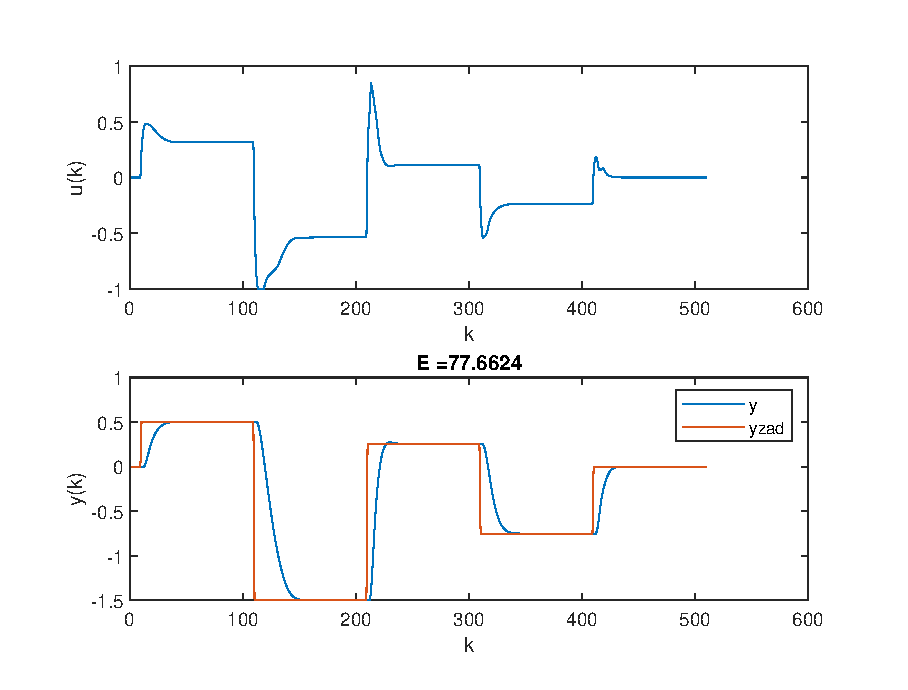
\includegraphics[width=0.8\linewidth]{img/strojenieNO_N_19_Nu_2_lam_4.eps}
			\caption{Działanie regulatora NO z nastawami N=19, Nu=2, $\lambda$=4}
			\label{fig:NO}
		\end{figure}
	\input{komendy.tex}

\end{document}